\documentclass[a4paper,UTF8]{article}
\usepackage{ctex}
\usepackage[margin=1.25in]{geometry}
\usepackage{color}
\usepackage{graphicx}
\usepackage{amssymb}
\usepackage{amsmath}
\usepackage{amsthm}
\usepackage{enumerate}
\usepackage{bm}
\usepackage{hyperref}
\usepackage{epsfig}
\usepackage{tikz}
\usepackage{color}
\usepackage{mdframed}
\usepackage{lipsum}
\usepackage{graphicx}

\newmdtheoremenv{thm-box}{Theorem}
\newmdtheoremenv{prop-box}{Proposition}
\newmdtheoremenv{def-box}{定义}
\usetikzlibrary{shapes.geometric, arrows}

\usepackage{listings}
\usepackage{xcolor}
\lstset{
	numbers=left, 
	numberstyle= \tiny, 
	keywordstyle= \color{ blue!70},
	commentstyle= \color{red!50!green!50!blue!50}, 
	frame=shadowbox, % 阴影效果
	rulesepcolor= \color{ red!20!green!20!blue!20} ,
	escapeinside=``, % 英文分号中可写入中文
	xleftmargin=2em,xrightmargin=2em, aboveskip=1em,
	framexleftmargin=2em
} 

\usepackage{booktabs}

\setlength{\evensidemargin}{.25in}
\setlength{\textwidth}{6in}
\setlength{\topmargin}{-0.5in}
\setlength{\topmargin}{-0.5in}
% \setlength{\textheight}{9.5in}
%%%%%%%%%%%%%%%%%%此处用于设置页眉页脚%%%%%%%%%%%%%%%%%%
\usepackage{fancyhdr}                                
\usepackage{lastpage}                                           
\usepackage{layout}                                             
\footskip = 10pt 
\pagestyle{fancy}                    % 设置页眉                 
\lhead{2018年春季}                    
\chead{机器学习导论}                                                
% \rhead{第\thepage/\pageref{LastPage}页} 
\rhead{作业三}                                                                                               
\cfoot{\thepage}                                                
\renewcommand{\headrulewidth}{1pt}  			%页眉线宽,设为0可以去页眉线
\setlength{\skip\footins}{0.5cm}    			%脚注与正文的距离           
\renewcommand{\footrulewidth}{0pt}  			%页脚线宽,设为0可以去页脚线

\makeatletter 									%设置双线页眉                                        
\def\headrule{{\if@fancyplain\let\headrulewidth\plainheadrulewidth\fi%
\hrule\@height 1.0pt \@width\headwidth\vskip1pt	%上面线为1pt粗  
\hrule\@height 0.5pt\@width\headwidth  			%下面0.5pt粗            
\vskip-2\headrulewidth\vskip-1pt}      			%两条线的距离1pt        
 \vspace{6mm}}     								%双线与下面正文之间的垂直间距              
\makeatother  

%%%%%%%%%%%%%%%%%%%%%%%%%%%%%%%%%%%%%%%%%%%%%%
\numberwithin{equation}{section}
%\usepackage[thmmarks, amsmath, thref]{ntheorem}
\newtheorem{theorem}{Theorem}
\newtheorem*{definition}{Definition}
\newtheorem*{solution}{Solution}
\newtheorem*{prove}{Proof}
\newcommand{\indep}{\rotatebox[origin=c]{90}{$\models$}}

\usepackage{multirow}

%--

%--
\begin{document}
\title{机器学习导论\\
作业三}
\author{151220129, 吴政亿, wuzy.nju@gmail.com}
\maketitle



\section{[15pts] Decision Tree I}

\begin{enumerate}[ {(}1{)}]
	\item \textbf{[5pts]} 假设一个包含三个布尔属性${X, Y, Z}$的空间,并且目标函数是$f(x,y,z) = x\ \mathbf{XOR}\ z$,其中$\mathbf{XOR}$为异或运算符。令$H$为基于这三个属性的决策树,请问:目标函数$f$可实现吗?如果可实现,画出相应的决策树以证明;如果不可实现,请论证原因;
	
	\item \textbf{[10pts]} 现有如表~\ref{table:ranking}所示数据集:
	
	\begin{table}[!h]
		\centering
		\caption{样例表} \vspace{2mm}\label{table:ranking}
		\begin{tabular}{c c c|c}\hline
			$X$ & $Y$ & $Z$ & $f$ \\
			\hline
			$1$ & $0$  & $1$ &  $1$\\
			$1$ & $1$  & $0$ &  $0$\\
			$0$ & $0$  & $0$ &  $0$\\
			$0$ & $1$  & $1$ &  $1$\\
			$1$ & $0$  & $1$ &  $1$\\
			$0$ & $0$  & $1$ &  $0$\\
			$0$ & $1$  & $1$ &  $1$\\
			$1$ & $1$  & $1$ &  $0$\\
			\hline
		\end{tabular}
	\end{table}
	
	请画出由该数据集生成的决策树。划分属性时要求以信息增益 (information gain)为准则。当信息增益 (information gain)相同时,依据字母顺序选择属性即可。
\end{enumerate}
\begin{solution}
	此处用于写解答(中英文均可)
	\begin{enumerate}[ {(}1{)}]
		\item 
		\thispagestyle{empty}
		% 定义基本形状
		\tikzstyle{results}=[ellipse ,text centered,draw=black]
		\tikzstyle{decisions} =[rectangle, rounded corners,text centered, draw = black]
		% 箭头形式
		\tikzstyle{arrow} = [-,>=stealth]
		\begin{tikzpicture}[node distance=1cm]
		%定义具体形状和相关位置
		\node[decisions](rootnode){ X$=?$ };
		\node[decisions,below of=rootnode,yshift=-0.5cm,xshift=-2cm](z1){ Z$=?$ };
		\node[decisions,below of=rootnode,yshift=-0.5cm,xshift=2cm](z2){ Z$=?$ };
		\node[results,below of=z1,yshift=-0.5cm,xshift=-1cm](result1){0};
		\node[results,below of=z1,yshift=-0.5cm,xshift=1cm](result2){1};
		\node[results,below of=z1,yshift=-0.5cm,xshift=3cm](result3){0};
		\node[results,below of=z1,yshift=-0.5cm,xshift=5cm](result4){1};
		%连接形状
		\draw [arrow] (rootnode) -- node [left,font=\small] {1} (z1);
		\draw [arrow] (rootnode) -- node [right,font=\small] {0} (z2);
		\draw [arrow] (z1) -- node [right,font=\small] {1} (result1);
		\draw [arrow] (z1) -- node [left,font=\small] {0} (result2);
		\draw [arrow] (z2) -- node [right,font=\small] {1} (result3);
		\draw [arrow] (z2) -- node [left,font=\small] {0} (result4);
		\end{tikzpicture}
		
		\item
		首先计算根节点的信息熵:\\
		$$	Ent(D) = - \sum^{|\gamma|}_{k=1}{p_k\log_2{p_k}}
			=-(\frac{1}{2}\log_2{\frac{1}{2}}+\frac{1}{2}\log_2{\frac{1}{2}})=1$$
		然后计算每个属性的信息增益:\\
		\begin{equation*}
		\begin{aligned}
		&Gain(D,\mathbf{X}) &=& 0;\\
		&Gain(D,\mathbf{Y}) &=& 0;\\
		&Gain(D,\mathbf{Z}) &=& 1-\frac{6}{8}*(-\frac{4}{6}\log_2{\frac{4}{6}}+\frac{2}{6}\log_2{\frac{2}{6}})-\frac{2}{6}*0=0.311;
		\end{aligned}			
		\end{equation*}
		显然,$\mathbf{Z}$的信息增益最大,于是他被选为划分属性。\\
		当$\mathbf{Z}=0$时,$f$都等于1,当$\mathbf{Z}=1$时,可见应用$\mathbf{X}$与$\mathbf{Y}$的信息增益相同,因此根据字母顺序选择$\mathbf{X}$作为划分属性。
		
		\thispagestyle{empty}
		% 定义基本形状
		\tikzstyle{results}=[ellipse ,text centered,draw=black]
		\tikzstyle{decisions} =[rectangle, rounded corners,text centered, draw = black]
		% 箭头形式
		\tikzstyle{arrow} = [-,>=stealth]
		\begin{tikzpicture}[node distance=1cm]
		%定义具体形状和相关位置
		\node[decisions](rootnode){ $\mathbf{Z}=?$ };
		\node[decisions,below of=rootnode,yshift=-0.5cm,xshift=-2cm](x){ $\mathbf{X}=?$ };
		\node[decisions,below of=x,yshift=-0.5cm,xshift=-2cm](y1){ $\mathbf{Y}=?$ };
		\node[decisions,below of=x,yshift=-0.5cm,xshift=2cm](y2){ $\mathbf{Y}=?$ };
		\node[results,below of=rootnode,yshift=-0.5cm,xshift=2cm](result0){0};
		\node[results,below of=y1,yshift=-0.5cm,xshift=-1cm](result1){0};
		\node[results,below of=y1,yshift=-0.5cm,xshift=1cm](result2){1};
		\node[results,below of=y1,yshift=-0.5cm,xshift=3cm](result3){1};
		\node[results,below of=y1,yshift=-0.5cm,xshift=5cm](result4){0};
		%连接形状
		\draw [arrow] (rootnode) 	-- node [left,font=\small] 	{1} (x);
		\draw [arrow] (rootnode) 	-- node [right,font=\small] {0} (result0);
		\draw [arrow] (x) 			-- node [left,font=\small] 	{1} (y1);
		\draw [arrow] (x) 			-- node [right,font=\small] {0} (y2);
		\draw [arrow] (y1) 			-- node [left,font=\small] 	{1} (result1);
		\draw [arrow] (y1) 			-- node [right,font=\small] {0} (result2);
		\draw [arrow] (y2) 			-- node [left,font=\small] 	{1} (result3);
		\draw [arrow] (y2) 			-- node [right,font=\small] {0} (result4);
		\end{tikzpicture}
		
	\end{enumerate}
\end{solution}
\newpage



 \section{[20pts] Decision Tree II}
 考虑如下矩阵:
 $$
 \begin{bmatrix}
 4 & 6 & 9 & 1 & 7 & 5 \\
 1 & 6 & 5 & 2 & 3 & 4
 \end{bmatrix}^T
 $$

 该矩阵代表了$6$个样本数据,每个样本都包含$2$个特征$f_1$和$f_2$。这$6$个样本数据对应的标签如下:
 $$
 \begin{bmatrix}
 1 & 0 & 1 & 0 & 1 & 0
 \end{bmatrix}^T
 $$

 在这个问题中,我们要构造一个深度为$2$的树进行分类任务。

 \begin{enumerate}[ {(}1{)}]
 	\item \textbf{[5pts]} 请计算根结点 (root) 的熵值 (entropy);

 	\item \textbf{[10pts]} 请给出第一次划分的规则,例如$f_1 \geq 4, f_2 \geq 3$。对于第一次划分后产生的两个结点,请给出下一次划分的规则;

 	提示:可以直观判断,不必计算熵。

 	\item \textbf{[5pts]} 现在回到根结点 (root),并且假设我们是建树的新手。是否存在一种划分使得根结点 (root) 的信息增益 (information gain) 为$0$?
 \end{enumerate}

 \begin{solution}
 	此处用于写解答(中英文均可)
 	\begin{enumerate}[ {(}1{)}]
 		\item 首先计算根节点的信息熵:\\
 		$$	Ent(D) = - \sum^{|\gamma|}_{k=1}{p_k\log_2{p_k}}
 		=-(\frac{1}{2}\log_2{\frac{1}{2}}+\frac{1}{2}\log_2{\frac{1}{2}})=1$$
 		
 		\item 		\thispagestyle{empty}
 		% 定义基本形状
 		\tikzstyle{results}=[ellipse ,text centered,draw=black]
 		\tikzstyle{decisions} =[rectangle, rounded corners,text centered, draw = black]
 		% 箭头形式
 		\tikzstyle{arrow} = [-,>=stealth]
 		\begin{tikzpicture}[node distance=1cm]
 		%定义具体形状和相关位置
 		\node[decisions](rootnode){ $f_1=?$ };
 		\node[decisions,below of=rootnode,yshift=-0.5cm,xshift=-2cm](lchildnode){ $f_2=?$ };
 		\node[results,below of=rootnode,yshift=-0.5cm,xshift=2cm](result1){0};
 		\node[results,below of=lchildnode,yshift=-0.5cm,xshift=-1cm](result2){1};
 		\node[results,below of=lchildnode,yshift=-0.5cm,xshift=1cm](result3){0};
 		%连接形状
 		\draw [arrow] (rootnode) 	-- node [left,font=\small] 	{$f_1\leq6$} 	(lchildnode);
 		\draw [arrow] (rootnode) 	-- node [right,font=\small] {$f_1>6$} 		(result1);
 		\draw [arrow] (z1) 			-- node [left,font=\small] 	{$f_2\geq2$} 	(result2);
 		\draw [arrow] (z1) 			-- node [right,font=\small] {$f_2<2$} 		(result3);
 		\end{tikzpicture}
 		
 		\item 可以。我们根据$f_1 \leq 4$($f_2 \leq 2$,$f_2 \leq 4$也行)来划分,可以得到两个子集:\\
 		$D^1(f_1 \leq 4)$,$D^1(f_1 > 4)$。\\
 		计算他们各自的信息熵为:\\
 		\begin{equation*}
 		\begin{aligned}
		Ent(D^1)&=&-(\frac{1}{2}\log_2{\frac{1}{2}}+\frac{1}{2}\log_2{\frac{1}{2}})=1\\	Ent(D^2)&=&-(\frac{1}{2}\log_2{\frac{1}{2}}+\frac{1}{2}\log_2{\frac{1}{2}})=1
 		\end{aligned}			
 		\end{equation*}
 		信息增益为:
 		$$Gain(D,f_1) = Ent(D)-\sum_{v=1}^2{\frac{|D^v|}{|D|}Ent(D^v)}\\
 		=1-(\frac{2}{6}*1+\frac{4}{6}*1)=0$$
 	\end{enumerate}
 \end{solution}
\newpage

 \section{[25pts] Universal Approximator}
 已知函数$f:[-1, 1]^n \mapsto [-1, 1]$满足$\rho$-Lipschiz性质。 给定误差$\epsilon > 0$,请构造一个激活函数为\mbox{ sgn($\mathbf{x}$) }的神经网络$ \mathcal{N}:[-1,1]^n \mapsto [-1,1] $,使得对于任意的输入样本$ \mathbf{x} \in [-1,1]^n $,有$|f(\mathbf{x}) - \mathcal{N}(\mathbf{x})| \leq \epsilon$。\\
 (Lipschiz条件为:$ \forall \mathbf{x}, \mathbf{y} \in [-1,1]^n$,$ \exists \rho > 0$,$ \mbox{ s.t. } |f(\mathbf{x})-f(\mathbf{y})| \leq \rho \lVert \mathbf{x} - \mathbf{y} \rVert_2 $,其中\mbox{ sgn($\mathbf{x}$) }的定义参见《机器学习》第98页。)
 
  \begin{enumerate}[ {(}1{)}]
 	\item \textbf{[5pts]} 请画出构造的神经网络$\mathcal{N}$的示意图;
 	
 	\item \textbf{[10pts]} 请对构造的神经网络进行简要的说明(写清每一层的线性组合形式,也就是结点间的连接方式和对应的权重);
 	
 	\item \textbf{[10pts]} 证明自己构造的神经网络的拟合误差满足要求。
 \end{enumerate}


 \begin{solution}
	此处用于写解答(中英文均可)
	\begin{enumerate}[ {(}1{)}]
		\item 见图\ref{p30}
		 	\begin{figure}[!h]
				\centering   
				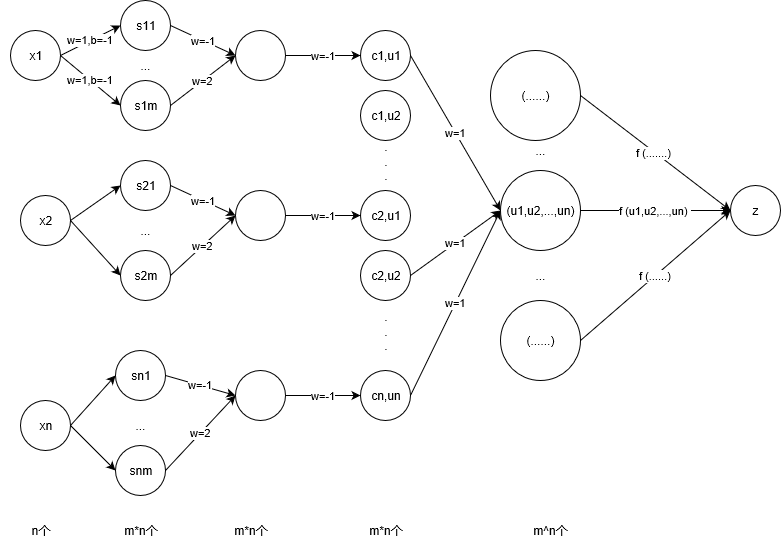
\includegraphics[width=1\textwidth, height=0.85\textwidth]{p30.png}  
				\caption{神经网络$\mathcal{N}$的示意图} 
				\label{p30}
			\end{figure}
		\pagebreak
		
		\item 首先给出阶跃函数的定义,其中当$x=0$时取值为$1$:
		 $$sgn(x) = \begin{cases}
		 1& \text{,$x \geq 0$}\\
		 0& \text{,$x < 0$}
		 \end{cases}$$
		 计算值:$$y = wx-b$$
		 对于函数$\mathcal{N}$的其中一个维度,我们将其划分为m份,则其被划分为$[-1,\frac{2}{m}],......,[1-\frac{2}{m},1]$,那么我们就可以将定义域划分为$m^n$个子空间。\\
		 我们首先构造一个神经元模型用于确定输入$x_i$在m的哪一个子空间中,见图\ref{p31}。\\
		 
		 \begin{figure}[!h]
		 	\centering   
		 	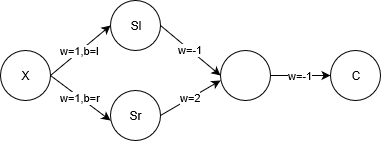
\includegraphics[width=0.8\textwidth, height=0.3\textwidth]{p31.png}  
		 	\caption{判断$x_k$是否在子空间$[l,r]$中} 
		 	\label{p31}
		 \end{figure}
	 %	\pagebreak
	 	这个神经元网络模型可以判断$x_k$是否在子空间$[l,r]$中,因此我们对于输入$x$可以构造n个此结构得到输出$c_1,...,c_n$,这是一个输出只有1和0的序列,并且只有一个$c_i=1$,其余均为0。\\
	 	接下来,我们应用这个子模型构造一个模型来得到样本x在哪一个子空间中($m^n$个),见图\ref{p32},定义子域为$(c_1,c_2,...,c_m)$,\\
	 	$c_i \in \{1,2,...,n\}$,$W_{ij}(i=\{1,...,n\},j=\{1,...,m\})$代表x的第i的参数$c_i$位于第j个子域中。它的Sgn(·)函数为:
	 	$$Sgn(\cdot) = \sum_{i=1}^n{w_ix_i}-n=\sum_{i=1}^n{W_{ic_i}}-n$$
	 	
	 	\begin{figure}[!h]
	 		\centering   
	 		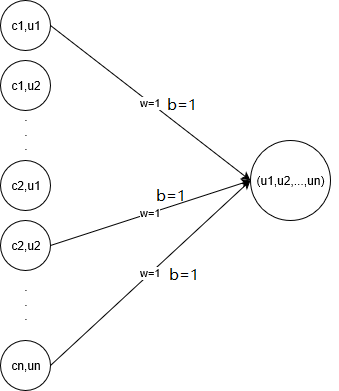
\includegraphics[width=0.5\textwidth, height=0.5\textwidth]{p32.png}  
	 		\caption{判断样本x是否在子域空间$(u_1,...,u_n)$中} 
	 		\label{p32}
	 	\end{figure}
	 	
	 	
	 %	\pagebreak
	 	那么对于$m^n$个隐层神经元也是一个只有一个取值为1,其他都是0的输入,我们令每一个子域它对应的取值时它中心在函数$f$上的取值,定义$u = \frac{l+r}{2}$。我们只需要给每一个输出设置权重为$f(u_1,u_2,...,u_n)$,便可以得到神经网络$\mathcal{N}$的输出,见图\ref{p33}。
	 	
	 	\begin{figure}[!h]
	 		\centering   
	 		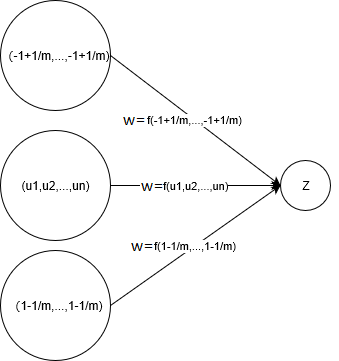
\includegraphics[width=0.5\textwidth, height=0.5\textwidth]{p33.png}  
	 		\caption{根据子域计算最终输出$\mathcal{N}$} 
	 		\label{p33}
	 	\end{figure}
 		
 	%	\pagebreak
 		\item 对于任意的输入样本$ \mathbf{x} \in [-1,1]^n, \exists \rho > 0$,对于$x_i$,
 		由于求值的点在子域的中心,因此有\\
 		$|u_i-x_i|\leq \frac{1}{m}$,故
 		$$
 		|f(\mathbf{x}) - \mathcal{N}(\mathbf{x})| 
 		\leq \rho\sqrt{\sum_{i=1}^{n}{(u_i-x_i)^2}}\\
 		\leq \rho\sqrt{n(\frac{1}{m}^2)}\\
 		\leq \epsilon
 		$$
 		得到当m满足下式时,符合条件。
 		$$m \geq \frac{\rho\sqrt{n}}{\epsilon}$$
 		另外,可以得到结论,随着m的增加,神经网络$\mathcal{N}$的拟合度将越来越高,由此可见,无论什么函数,只要他是连续的,应用神经网络都可以拟合得到令人满意的结果。
	\end{enumerate}
\footnote{\textbf{在本题的solution中,我要特别致谢陆依鸣同学,他给我提供了宝贵无比的思路,也要致谢吴昕,她在本题的神经网络结构中给予了巨大的帮助。}}
 \end{solution}
\pagebreak
\newpage

\section{[40pts] Neural Network in Practice}
通过《机器学习》课本第5章的学习,相信大家已经对神经网络有了初步的理解。深度神经网络在某些现实机器学习问题,如图像、自然语言处理等表现优异。本次作业旨在引导大家学习使用一种深度神经网络工具,快速搭建、训练深度神经网络,完成分类任务。

我们选取PyTorch为本次实验的深度神经网络工具,有了基础工具,我们就能如同搭积木一样构建深度神经网络。\href{http://pytorch.org/}{PyTorch}是Facebook开发的一种开源深度学习框架,有安装方便、文档齐全、构架方便、训练效率高等特点。本次作业的首要任务就是安装PyTorch。

目前PyTorch仅支持Linux和MacOS操作系统,所以Window用户需要装一个Linux虚拟机或者直接安装Linux系统。PyTorch安装很方便,只需要在其主页中的Get Start一栏选择对应的环境设置,便能够一键安装。有GPU的同学也可以尝试安装GPU版本的PyTorch。为保证此次作业的公平性,只要求使用CPU进行网络训练,当然有条件的同学也可以尝试使用GPU进行训练。在批改作业时,助教会提供Python 2.7、3.5、3.6三种环境进行实验验证。

我们选取CIFAR10作为本次作业的训练任务。\href{https://en.wikipedia.org/wiki/CIFAR-10}{CIFAR10}是一个经典的图片分类数据集,数据集中总共有60000张32$\times$32的彩色图片,总共有10类,每类6000张图片,其中50000张图片构成训练集,10000张图片构成测试集。PyTorch通过torchvision给用户提供了获取CIFAR10的方法,详细信息可见\href{http://pytorch.org/tutorials/beginner/blitz/cifar10_tutorial.html}{PyTorch的教程}。此外关于CIFAR10分类准确率排行可见此\href{http://rodrigob.github.io/are_we_there_yet/build/classification_datasets_results.html}{链接}。

下面我们将尝试使用PyTorch来解决实际问题:

\begin{enumerate}[(1)]
	\item \textbf{[15pts]} 首先我们跟随PyTorch的教程,用一个简单的卷积神经网络(Convolutional Neural Network, CNN),完成CIFAR10上的分类任务,具体要求如下:
	
	\begin{itemize}
		\item \textbf{[7pts]} 在代码实现之前,大家可能需要对CNN网络进行一定的了解,请大家自行查阅资料(PyTorch的教程中也有部分介绍CNN网络),并在实验报告中给出对CNN的见解:主要回答什么是卷积层,什么是Pooling层,以及两者的作用分别是什么;
		\item \textbf{[8pts]} 接下来就是具体的代码实现和训练。教程会手把手教你完成一次训练过程,其中使用SGD作为优化方法,请同学们自行调整epoch的大小和学习率,完成此次训练。另外,请在实验报告中给出必要的参数设置,以及训练结果如最终的loss、在测试集上的准确率等;
	\end{itemize}
	\item \textbf{[20pts]} 显然,这样一个简单的网络在CIFAR10上并不能取得令人满意的结果,我们需要选取一个更为复杂的网络来提升训练效果。在此小题中,我们选取了CIFAR10准确率排行榜上排名第二的结构,具体参见\href{https://arxiv.org/pdf/1412.6806.pdf}{论文链接}。为了方便大家实现,我们直接给出了网络结构如图\ref{network_structure}所示。请大家搭建完成此网络结构,并选择Adam为优化器,自行调整相关参数完成训练和预测,实验结果报告内容同第(1)小题;
	\begin{figure}[!h]
		\centering   
		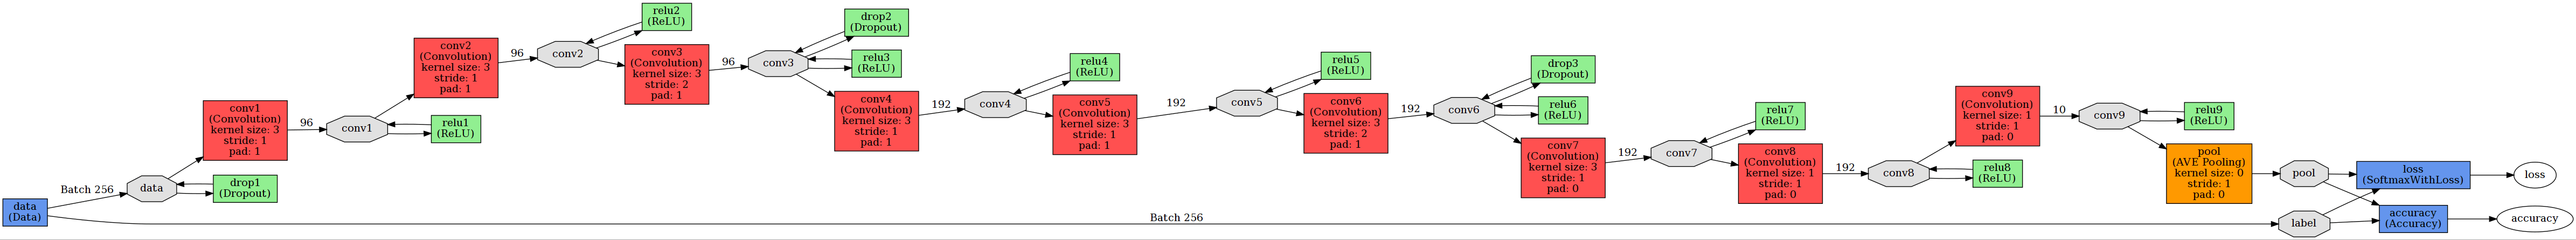
\includegraphics[width=0.99\textwidth,height=0.15\textwidth]{nn_structure.png}  
		\caption{待实现网络结构} 
		\label{network_structure}
	\end{figure}
	\item \textbf{[5pts]} 通过上一题实验我们可以发现,即使使用现成的网络结构也不一定能达到与其相同的训练效果。请大家分析其中的原因,并谈谈本次实验的感想,以及对深度学习调参的体会。
\end{enumerate}

\noindent{\textbf{实验报告.}}
\begin{enumerate}[(1)]
	\item 
	\subsection{卷积神经网络简介}
	卷积神经网络(Convolutional Neural Network, CNN)是一种前馈神经网络,它的人工神经元可以响应一部分覆盖范围内的周围单元,对于大型图像处理有出色表现。卷积神经网络与普通神经网络的区别在于,卷积神经网络包含了一个由卷积层和子采样层构成的特征抽取器。在卷积神经网络的卷积层中,一个神经元只与部分邻层神经元连接。在CNN的一个卷积层中,通常包含若干个特征平面(featureMap),每个特征平面由一些矩形排列的的神经元组成,同一特征平面的神经元共享权值,这里共享的权值就是卷积核。卷积核一般以随机小数矩阵的形式初始化,在网络的训练过程中卷积核将学习得到合理的权值。共享权值(卷积核)带来的直接好处是减少网络各层之间的连接,同时又降低了过拟合的风险。子采样也叫做池化(pooling),通常有均值子采样(mean pooling)和最大值子采样(max pooling)两种形式。子采样可以看作一种特殊的卷积过程。卷积和子采样大大简化了模型复杂度,减少了模型的参数。
	\subsection{定义介绍}
	卷积神经网络通常包含以下几种层:\\
	\begin{enumerate}
		\item \textbf{卷积层(Convolutional layer)},卷积神经网路中每层卷积层由若干卷积单元组成,每个卷积单元的参数都是通过反向传播算法优化得到的。卷积运算的目的是提取输入的不同特征,第一层卷积层可能只能提取一些低级的特征如边缘、线条和角等层级,更多层的网络能从低级特征中迭代提取更复杂的特征。
		\item \textbf{线性整流层(Rectified Linear Units layer, ReLU layer)},这一层神经的活性化函数(Activation function)使用线性整流(Rectified Linear Units, ReLU)$f(x)=max(0,x)$
		\item \textbf{池化层(Pooling layer)},通常在卷积层之后会得到维度很大的特征,将特征切成几个区域,取其最大值或平均值,得到新的、维度较小的特征。
		\item \textbf{全连接层( Fully-Connected layer)}, 把所有局部特征结合变成全局特征,用来计算最后每一类的得分。
	\end{enumerate}
	\subsection{卷积层}
	卷积层有两个重要的概念:
	\begin{enumerate}
		\item local receptive fields (感受视野)
		\item shared weights (共享权值)
	\end{enumerate}
	在神经网络中,隐藏层与输入层是全连接,对于本数据集来说就是$32*32*3=3072$的三维神经元,如果隐藏神经元有15个,那么参数个数就有$3072*15=46080$个,这个参数过于巨大了。而local receptive fields的意义就在于大幅度减少参数的个数,并且依旧拥有出色的性能。假设我们定义一个$5*5*3$的一个local receptive fields(三维的,因为RGB图像),即隐藏层的神经元与输入层的$5*5*3$个神经元相连,这可以类似看作隐藏层中的神经元 具有一个固定大小的感受视野去感受上一层的部分特征。在全连接神经网络中,隐藏层中的神经元的感受视野足够大乃至可以看到上一层的所有特征。\\
	而在卷积神经网络中,隐藏层中的神经元的感受视野比较小,只能看到上一次的部分特征,上一层的其他特征可以通过平移感受视野来得到同一层的其他神经元,由同一层其他神经元来看。假设每一次平移的stride(步长)为1,那么参数的个数就会锐减为$28*28=784$个。
	
	\subsection{池化层,"汇合"层}
	如果在卷积层选的local receptive fields和stride都比较小,得到的参数feature map依旧比较大,而池化层的意义就在于他可以对每一个feature map进行降维操作,同时深度依旧是feature map的个数保持不变。\\
	池化层也有一个类似于卷积层的"池化视野(filter)"来对feature map进行扫描降维度,一般有两种计算方式:
	\begin{enumerate}
		\item Max pooling: 取“池化视野”矩阵中的最大值
		\item Average pooling: 取“池化视野”矩阵中的平均值
	\end{enumerate}
	如果我们假定filter为2*2,stride为2的话,我们的feature map大小就会从784锐减到到$14*14=196$个。可见其作用是基于局部相关性原理进行亚采样,从而在减少数据量的同时保留有用信息。
	
	\subsection{实验参数}
	实验一中,我设置的参数是lr=0.001, momentum=0.9, weight\_decay=0.001,下列数据是一个具有代表性意义的典型特征结果。一系列可靠结果表明,该模型在准确率达到65\%左右便达到了最佳拟合状态,在后面的epoch中loss已经不再下降甚至令模型过拟合。下表~\ref{figure1}, ~\ref{p1.2}给出了epoch=15与epoch=50的对比,可以发现epoch=50得到的实验结果并没有前者优秀。\\
	
	大量具有重复性的精确良好实验均证明,epoch=15时模型达到最优,如图~\ref{p1.3}所示,不难得到如果我们将learn rate进一步调小,该模型的准确率还会有一定上升。
	\begin{table}[!h]
		\centering
		\caption{lr=0.001, momentum=0.9, weight\_decay=0.001, epoch=15}
		\label{figure1}
		\begin{tabular}{|c|c|c|c|c|c|c|c|c|c|c|}
			\hline
			Class          & plane & car  & bird & cat  & deer & dog  & frog & horse & ship & truck \\ \hline
			Accuracy       & 80\%  & 65\% & 53\% & 37\% & 60\% & 60\% & 79\% & 70\%  & 71\% & 71\%  \\ \hline
			Total accuracy & \multicolumn{10}{c|}{65\%}                                             \\ \hline
			Total loss 	   & \multicolumn{10}{c|}{2643}                                             \\ \hline
		\end{tabular}
	\end{table}

	\begin{table}[!h]
	\centering
	\caption{lr=0.001, momentum=0.9, weight\_decay=0.001, epoch=50}
	\label{p1.2}
	\begin{tabular}{|c|c|c|c|c|c|c|c|c|c|c|}
		\hline
		Class          & plane & car  & bird & cat  & deer & dog  & frog & horse & ship & truck \\ \hline
		Accuracy       & 66\%  & 89\% & 53\% & 37\% & 45\% & 62\% & 80\% & 59\%  & 75\% & 69\%  \\ \hline
		Total accuracy & \multicolumn{10}{c|}{64\%}                                             \\ \hline
		Total loss 	   & \multicolumn{10}{c|}{2807}                                             \\ \hline
	\end{tabular}
	\end{table}
	
	\begin{figure}[!h]
		\centering   
		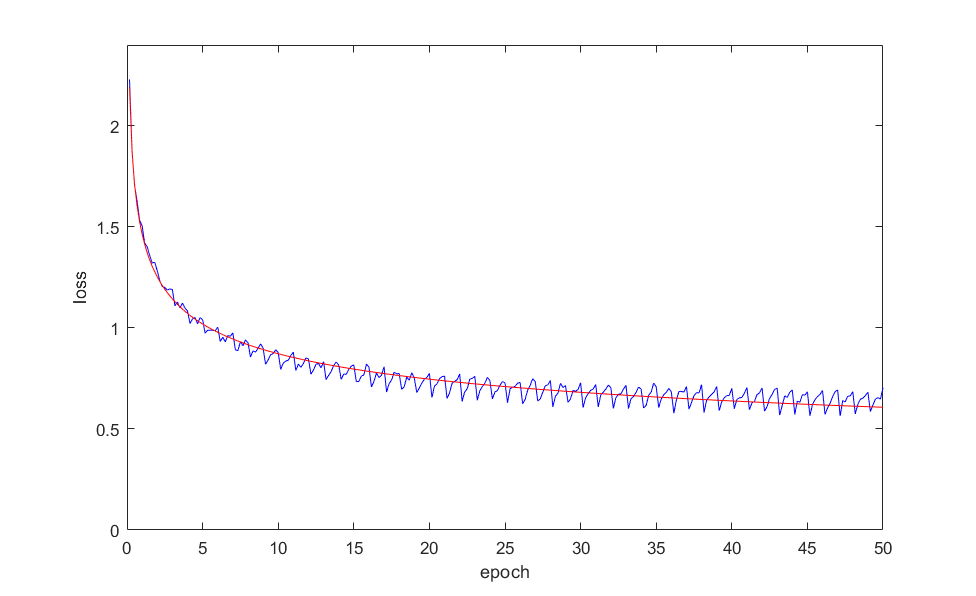
\includegraphics[width=0.5\textwidth, height=0.5\textwidth]{p1.png}  
		\caption{第一题:lr=0.001, momentum=0.9, weight\_decay=0.001} 
		\label{p1.3}
	\end{figure}
	
	\pagebreak
	\item 实验二中,大量的实验数据中,我选取了下列三组数据以展开进一步的分析。他们的学习率分别是0.001, 0.00025, 0.0001。观察表~\ref{p2.1}, ~\ref{p2.2}, ~\ref{p2.3}可以看出,学习率在0.00025时得到了较为出色的成绩,这个数据是从0.001到0.0001上随机分布然后实验后,得到的最为稳定下降的数值,可以观察图~\ref{p21}, ~\ref{p22}, ~\ref{p23}。至于更低的学习率与更高的epoch,由于每一次实验的时间代价过于昂贵,若想要得到得到更高的准确度,我们仍需在未来投入大量的工作并开展更为深入的研究。
	
	\begin{table}[!h]
		\centering
		\caption{lr = 0.001, weight\_decay=0.0001, epoch=50}
		\label{p2.1}
		\begin{tabular}{|c|c|c|c|c|c|c|c|c|c|c|}
			\hline
			Class          & plane & car  & bird & cat  & deer & dog  & frog & horse & ship & truck \\ \hline
			Accuracy       & 75\%  & 92\% & 84\% & 50\% & 69\% & 46\% & 66\% & 91\%  & 90\% & 94\%  \\ \hline
			Total accuracy & \multicolumn{10}{c|}{74\%}                                             \\ \hline
			Total loss 	   & \multicolumn{10}{c|}{29}                                             \\ \hline
		\end{tabular}
	\end{table}
	


	\begin{table}[!h]
	\centering
	\caption{lr = 0.00025, weight\_decay=0.0001, epoch=50}
	\label{p2.2}
	\begin{tabular}{|c|c|c|c|c|c|c|c|c|c|c|}
		\hline
		Class          & plane & car  & bird & cat  & deer & dog  & frog & horse & ship & truck \\ \hline
		Accuracy       & 81\%  & 100\% & 76\% & 31\% & 69\% & 53\% & 77\% & 83\%  & 95\% & 94\%  \\ \hline
		Total accuracy & \multicolumn{10}{c|}{77\%}                                             \\ \hline
		Total loss 	   & \multicolumn{10}{c|}{27}                                             \\ \hline
	\end{tabular}
	\end{table}

	\begin{table}[!h]
	\centering
	\caption{lr = 0.0001, weight\_decay=0.0001, epoch=50}
	\label{p2.3}
	\begin{tabular}{|c|c|c|c|c|c|c|c|c|c|c|}
		\hline
		Class          & plane & car  & bird & cat  & deer & dog  & frog & horse & ship & truck \\ \hline
		Accuracy       & 68\%  & 100\% & 76\% & 18\% & 53\% & 73\% & 66\% & 100\%  & 85\% & 76\%  \\ \hline
		Total accuracy & \multicolumn{10}{c|}{74\%}                                             \\ \hline
		Total loss 	   & \multicolumn{10}{c|}{28}                                             \\ \hline
	\end{tabular}
	\end{table}

	\begin{figure}[!h]
	\centering   
	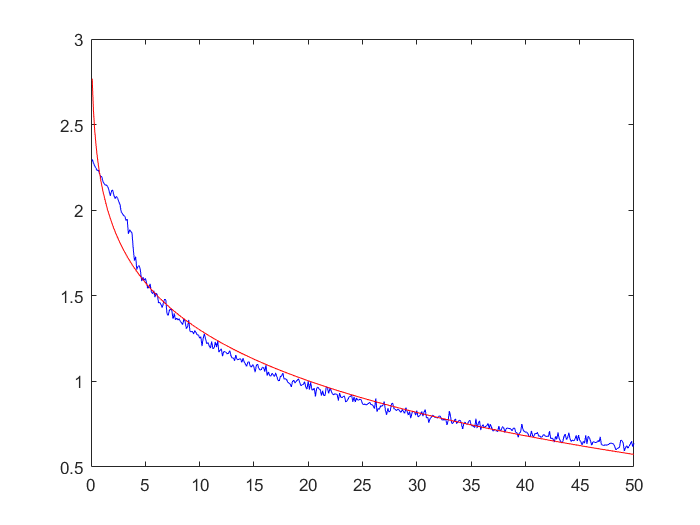
\includegraphics[width=0.5\textwidth, height=0.5\textwidth]{p21.png}  
	\caption{第二题:lr = 0.001, weight\_decay=0.0001, epoch=50} 
	\label{p21}
	\end{figure}

	\begin{figure}[!h]
	\centering   
	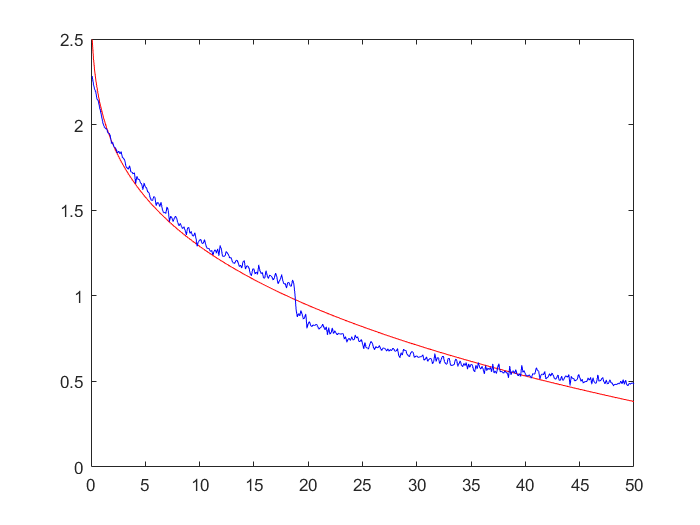
\includegraphics[width=0.5\textwidth, height=0.5\textwidth]{p22.png}  
	\caption{第二题:lr = 0.00025, weight\_decay=0.0001, epoch=50} 
	\label{p22}
	\end{figure}

	\begin{figure}[!h]
	\centering   
	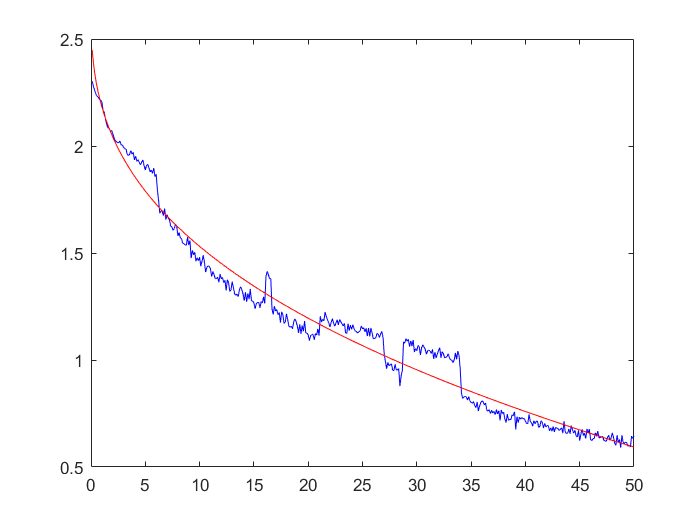
\includegraphics[width=0.5\textwidth, height=0.5\textwidth]{p23.png}  
	\caption{第二题:lr = 0.0001, weight\_decay=0.0001, epoch=50} 
	\label{p23}
	\end{figure}

	\pagebreak
	\item 
	在本次实验中,从理论上讲,我们可以得到近似论文中的准确率,然而事实上实验结果差强人意。这其中的误差可能源自一下几个方面:
	
	\begin{enumerate}
		\item 实验网络结构图中,最后一步pooling参数显示的kernel是0,但是实际上可能不是。
		\item 在相同的参数下,实验结果仍然具有一定的随机性,因此如果在实验条件允许的情况下,对于每一种参数取值都进行大量重复实验取平均值才可以准确判断这一模型的参数如何。
		\item 双方的学习率与epoch差别过大,论文作者也许lr取值远远小于或大于0.0001,这样的话逐步逼近也许会有着更好的结果,收敛时loss数值更低。	
	\end{enumerate}

	当然,本次实验中,我对于调参也有了一些体会,综合网上查到的一些资料,我列出了一些调参的方法:
	
	\begin{enumerate}
		\item 初始化。尝试不同的初始化方法可能对精度的影响巨大,例如用normal初始化cnn参数与xavier初始化参数。
		\item 进度条。良好的可视化可以帮助我们观察本次参数的取值如何,loss逐步下降与收敛可以告知我们机器学习的进度如何,是否要终止本次学习更新参数。
		\item Learning Rate合理。如果lr太大会导致loss爆炸,或者nan;如果lr太小会导致loss下降缓慢。对于lr的调参,如果我们观察到loss的数值从初始值一路下降,然后收敛到一定数值后,就意味着我们可以进一步降低学习率了。
		\item 可视化。将图片学习后可视化出来,如果发现和原始输入基本相同,那么很大程度就意味着feature map没有学到多少有价值的信息。
		\item weight可视化。通常,我们期待良好的卷积层的weight可视化出来会具备smooth的特性。如果发现图中有很多噪点,往往意味着我们的模型训练中出现了问题。
		\item 调参需要在验证集上,相比于训练集的loss,验证集的loss更为重要。
		\item \textbf{[玄学经验]一名合格的炼丹师,首先大力出奇迹,然后最后发现,你在训练模型的时候,模型也在训练你。}
	\end{enumerate}

\end{enumerate}
\footnote{\textbf{参考:https://www.cnblogs.com/muchen/p/6296957.html}}
\footnote{\textbf{参考:https://blog.csdn.net/cxmscb/article/details/71023576}}
\footnote{\textbf{参考:https://www.zhihu.com/question/25097993}}
\end{document}